\clearpage
\myparagraphold{\olly}
\myindex{\olly}

Let's try this example in \olly.
The input value of the function (2) is loaded into \EAX: 

\begin{figure}[H]
\centering
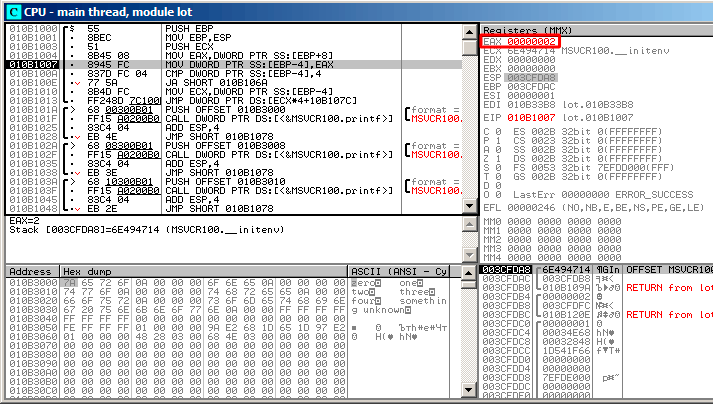
\includegraphics[scale=\FigScale]{patterns/08_switch/2_lot/olly1.png}
\caption{\olly: function's input value is loaded in \EAX}
\label{fig:switch_lot_olly1}
\end{figure}

\clearpage
The input value is checked, is it bigger than 4? 
If not, the \q{default} jump is not taken:
\begin{figure}[H]
\centering
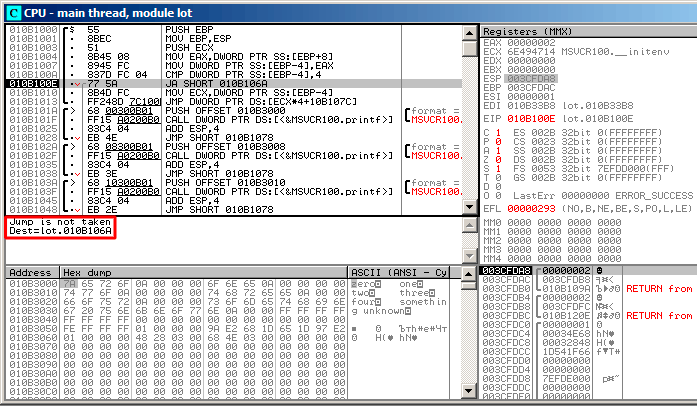
\includegraphics[scale=\FigScale]{patterns/08_switch/2_lot/olly2.png}
\caption{\olly: 2 is no bigger than 4: no jump is taken}
\label{fig:switch_lot_olly2}
\end{figure}

\clearpage
Here we see a jumptable:

\begin{figure}[H]
\centering
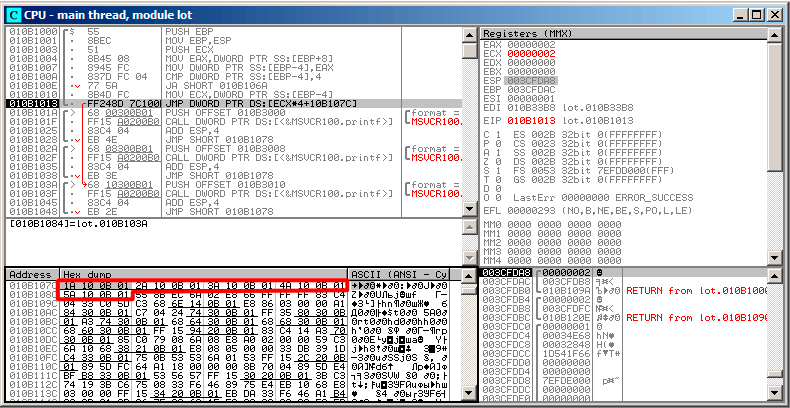
\includegraphics[scale=\FigScale]{patterns/08_switch/2_lot/olly3.png}
\caption{\olly: calculating destination address using jumptable}
\label{fig:switch_lot_olly3}
\end{figure}

Here we've clicked \q{Follow in Dump} $\rightarrow$ \q{Address constant}, so now we see the \IT{jumptable} in the data window.
These are 5 32-bit values\footnote{They are underlined by \olly because
these are also FIXUPs: \myref{subsec:relocs}, we are going to come back to them later}.
\ECX is now 2, so the second element (counting from zero) of the table is to be used.
It's also possible to click \q{Follow in Dump} $\rightarrow$ 
\q{Memory address} and \olly will show the element addressed by the \JMP instruction. 
That's \TT{0x010B103A}.

\clearpage
After the jump we are at \TT{0x010B103A}: the code printing \q{two} will now be executed:

\begin{figure}[H]
\centering
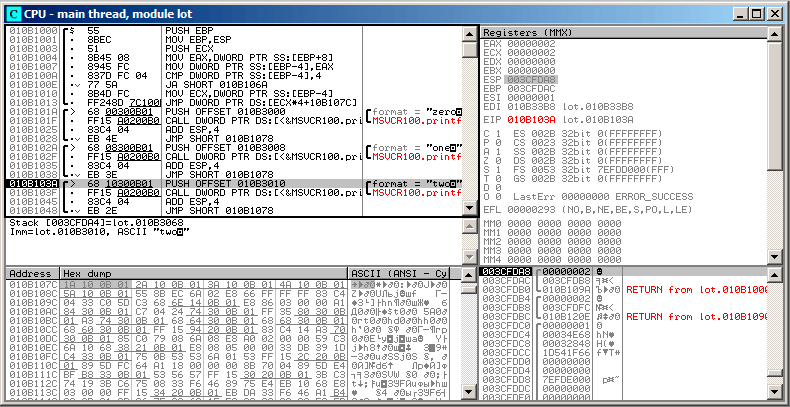
\includegraphics[scale=\FigScale]{patterns/08_switch/2_lot/olly4.png}
\caption{\olly: now we at the \IT{case:} label}
\label{fig:switch_lot_olly4}
\end{figure}
